\chapter{Le deep learning pour la vision artificielle}
\label{chap:deep-learning}
Nous nous intéressons ici au deep learning dans le cadre d'un apprentissage supervisé. Le but d'un réseau de neurones est de faire correspondre une base de données d'entrée (dans notre étude, des images) à une base de données de sortie (qui peut être des labels, une nouvelle image générée, une bounding box ou un pourcentage d'appartenance à une image). Le réseau ainsi construit peut être vu comme une fonction résolvant un problème particulier. Les deux types de réseaux sont les réseaux résolvant des problèmes de classification (catégoriser les entrées selon des valeurs discrètes correspondant à des classes définies) et ceux résolvant des problèmes de régression (évaluer des valeurs continues de sortie en fonction des valeurs d'entrée).

\section{Fonctionnement d'un neurone}
\label{sec:neurone}

Un \textit{neurone} est une entité informatique qui prend un vecteur de valeurs $\textbf{x} = (x_1, x_2, ..., x_d)$ en entrée pour retourner une valeur $y$ en sortie. Chaque $x_i$ est associé à un poids $w_i$ initialisé aléatoirement au départ. À l'intérieur du neurone, deux opérations sont exécutées. La première est la fonction de transfert $\Sigma = b + \sum{x_i \cdot w_i}$ où $b$ est une valeur nommée "biais". La deuxième est une fonction non-linéaire $f$ nommée "fonction d'activation" qui prend le résultat de la fonction de transfert en paramètre et retourne la sortie $y$. La figure \ref{fig:schema-neurone} illustre l'organisation d'un neurone. On peut résumer un neurone par l'équation suivante :
\begin{equation}
    y = f(\Sigma) = f(b + \sum_i{x_i \cdot w_i})
\end{equation}

\begin{figure}[!h]
\centering
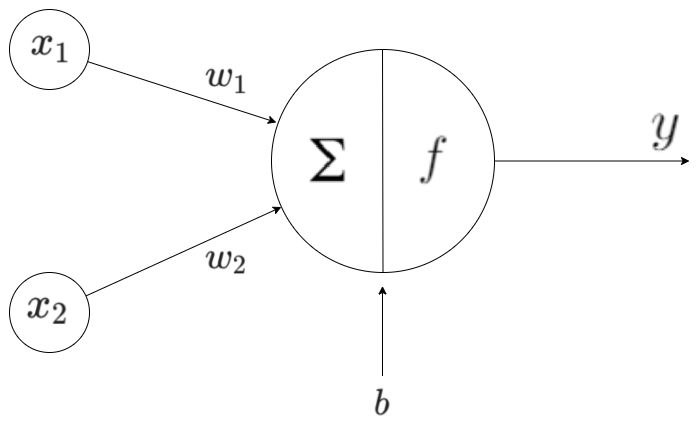
\includegraphics[scale=0.5]{img/neurone.PNG}
\caption{Schéma d'un neurone à deux entrées.}
\label{fig:schema-neurone}
\end{figure}

\section{Fonctionnement d'un réseau de neurones}
Plusieurs neurones connectés entre eux forment un \textit{réseau de neurones} (figure \ref{fig:exemple_network}). Les neurones sont regroupés par \textit{couches}. La première couche est appelée \textit{couche d'entrée}. Elle représente les valeurs que l'on fournit en entrée au réseau\footnote{Cette première couche n'effectue aucun calcul et se contente de passer les entrées à la couche suivante.}. La dernière couche est appelée \textit{couche de sortie}. Les résultats de cette couche sont les résultats finaux. Les autres couches sont les \textit{couches cachées}.

\begin{figure}[!h]
\centering
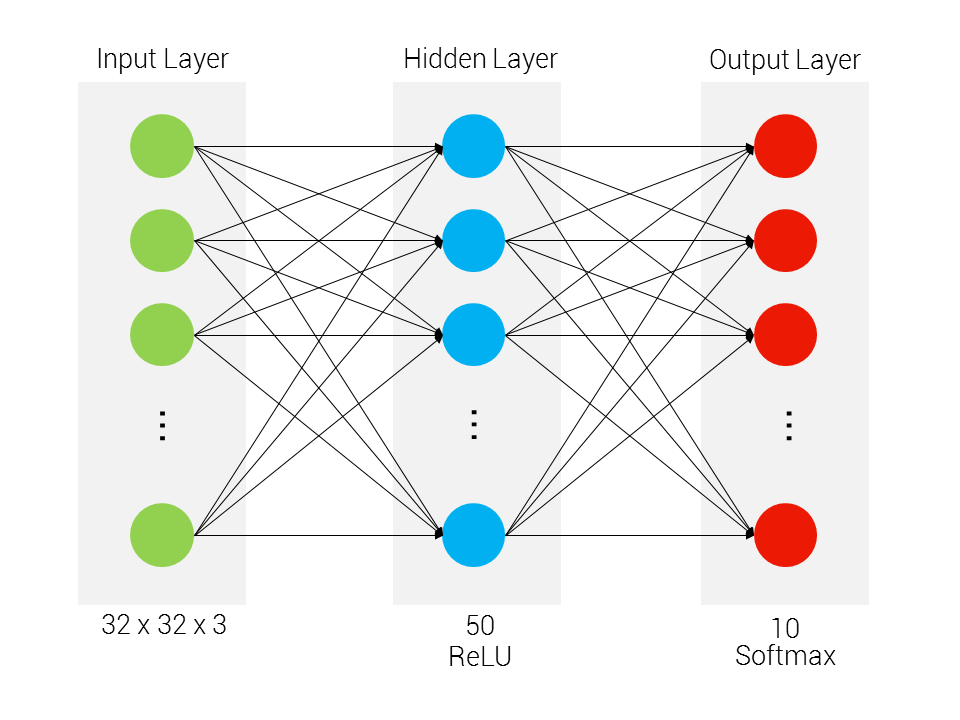
\includegraphics[scale=0.5]{img/neural_ex.png}
\caption{Exemple d'un réseau de neurones avec une couche d'entrée, une couche de sortie et une couche cachée. Source :  \url{https://ljvmiranda921.github.io/notebook/2017/02/17/artificial-neural-networks/}}
\label{fig:exemple_network}
\end{figure}

À l'initialisation, les poids et les biais des neurones sont choisis aléatoirement. L'ensemble des poids et des biais utilisés dans un réseau de neurones est noté $\theta$. Le but est de changer $\theta$ afin que le réseau fasse correspondre les entrées aux sorties. Cette phase de changement des paramètres s'appelle \textit{"phase d'entraînement"}. On utilise généralement une grande quantité de données annotées pour cette phase.

Pour entraîner un réseau, on effectue les tâches suivantes :
\begin{itemize}
  \item On entre des données dans le réseau par la couche d'entrée.
  \item On calcule  la "fonction de coût"\footnote{Loss, en anglais.}, qui permet d'évaluer la différence entre les sorties du réseau de neurones et ce qui était attendu.
  \item On utilise une "fonction d'optimisation" (par exemple, la descente du gradient) qui permet de corriger petit à petit les poids pour minimiser la fonction de coût, grâce à la \textit{rétro-propagation} ("backpropagation", en anglais) de la fonction de coût.
\end{itemize}

% TODO
La \textit{backpropagation} consiste à appliquer une fonction qui propage l'erreur entre la prédiction et le résultat attendu. Les poids de chaque couche et des liens sont corrigés en partant de la couche de sortie puis en remontant jusqu'à la couche d'entrée.

\section{Réseau de neurones convolutionnel}

\begin{figure}[!h]
\centering
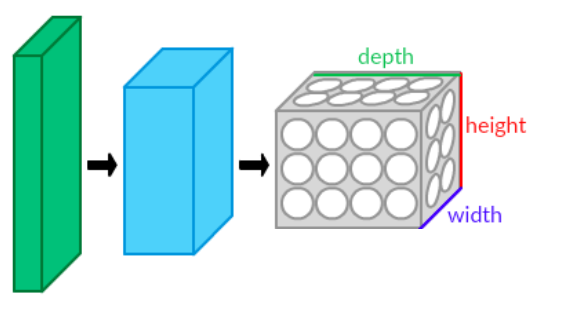
\includegraphics[scale=0.4]{img/Conv_layers.png}
\caption{Illustration d'une couche de convolution d'un CNN. La couche verte montre le volume des entrées, la couche bleue montre la couche de neurones construite en filtres de convolution (avec une profondeur). Après la convolution du volume d'entrée par la couche de convolution, on obtient le volume de sortie, en gris, dont la largeur, la hauter et la profondeur ont été modifiées. Source : \url{https://www.wikiwand.com/fr/R\%C3\%A9seau_neuronal_convolutif}}
\label{fig:cnn-layer}
\end{figure}

Les réseaux de neurones classiques fonctionnent mal en vision artificielle, pour la raison que les données en entrée sont des images, c'est-à-dire des tenseurs de $W \times H \times 3$ pixels pour des images couleurs RGB de largeur $W$ et de hauteur $H$, par exemple. Un réseau de neurones classique ne permet pas de retenir la notion de structure géométrique des pixels dans une image, ce qui aboutit à des performances peu convaincantes en vision artificielle.

Les réseaux de neurones convolutionnels (CNN\footnote{Convolutional Neural Network}, en abrégé) sont une variante des réseaux de neurones qui permettent de répondre à ce problème et qui sont la brique de base des solutions de deep learning en vision par ordinateur. Les CNNs sont composés de \textit{couches de convolutions}, des couches où les neurones sont organisés à la manière de filtres de convolutions sur les données d'entrée. La figure \ref{fig:cnn-layer} illustre brièvement le fonctionnement d'une couche de convolution.

Des recherches \cite{CNN-visu} ont montré que ces couches de convolution permettent de calculer et récupérer des caractéristiques de l'image. Les premières couches de convolution retirent des caractéristiques bas-niveau (contours, par exemple) tandis que les couches plus profondes sont sensibles à des caractéristiques plus haut-niveau. La figure \ref{fig:features-cnn} illustre l'apprentissage de ces caractéristiques en fonction de la profondeur des couches.

\begin{figure}[!h]
\centering
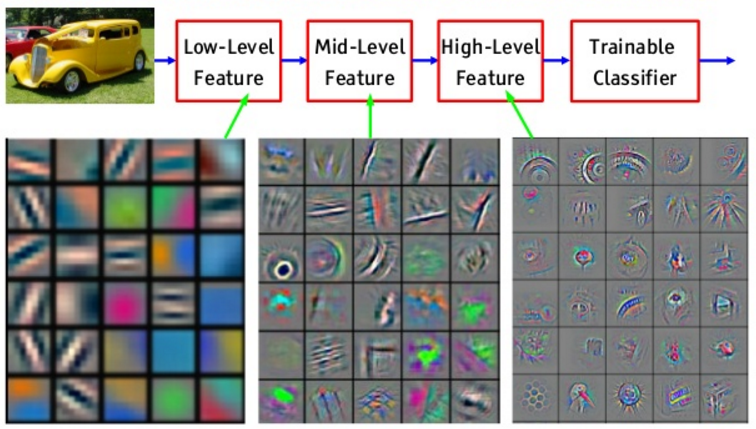
\includegraphics[scale=0.4]{img/cnn-vizzzz.png}
\caption{Illustration des caractéristiques de l'image extraites par un CNN. Des caractéristiques bas-niveau comme des contours sont extraites dans les couches les moins profondes. Puis, des caractéristiques de plus en plus haut niveau sont apprises au fur et à mesure que les couches sont profondes. Source : \url{https://medium.com/@kalfasyan/my-connectionist-approach-to-deep-learning-part-1-a9b190356295}}
\label{fig:features-cnn}
\end{figure}

\section{Définition d'un ensemble de données pour réseau de neurones}
En général, l'ensemble de données (ou "dataset", en anglais) qui traite un problème de vision artificielle contient :
\begin{itemize}
    \item \textbf{Ensemble d'apprentissage :} de nombreuses images supervisées, annotées à la main. Cet ensemble est destiné à faire apprendre au modèle.
    
    \item \textbf{Ensemble de test :} un ensemble (plus petit que l'ensemble d'apprentissage) d'images supervisées. Ces images vont servir à mesurer les performances du réseau après que celui-ci ait été entraîné sur l'ensemble d'apprentissage.
\end{itemize}

\hspace{1pt}
\par\noindent\rule{\textwidth}{0.4pt}
 
Ce chapitre permet au lecteur de prendre connaissance des bases des réseaux de neurones dont nous nous servons dans ce rapport. Ce sont ces bases qui sont, encore aujourd'hui, les fondations de l'application du deep learning dans les tâches de vision par ordinateur. Nous voyons dans le chapitre suivant comment ce principe du deep learning est exploité pour résoudre les tâches de vision artificielle rencontrées dans ce projet.